% IAM-XAI -- IEEE conference paper draft
% Compile with pdfLaTeX + BibTeX (e.g. upload the whole paper/ folder to Overleaf).
% Every number below comes from evaluation/RESULTS.md (regenerate with
% `python -m experiments.summary`); do not edit numbers by hand.
\documentclass[conference]{IEEEtran}
\IEEEoverridecommandlockouts

\usepackage{cite}
\usepackage{amsmath,amssymb,amsfonts}
\usepackage{graphicx}
\usepackage{textcomp}
\usepackage{xcolor}
\usepackage{booktabs}
\usepackage{multirow}
\usepackage{tikz}
\usetikzlibrary{arrows.meta,positioning}
\usepackage{url}
\usepackage[hidelinks]{hyperref}

\graphicspath{{figures/}}
\newcommand{\todo}[1]{\textcolor{red}{[#1]}}
\newcommand{\code}[1]{\texttt{#1}}

\begin{document}

\title{IAM-XAI: Explainable Attack Path Risk Assessment for Cloud Identity Configurations}

\author{
\IEEEauthorblockN{Alan Chris Dsilva, Anna Mariya Jose, Bharathan K and Dr. Julian Benedit P}
\IEEEauthorblockA{\textit{Dept. of Computer Science and Engineering} \\
\textit{CHRIST (Deemed to be University)}, Bengaluru, India \\
alanchrisdisilva@gmail.com, annamariya2605@gmail.com, bytexbharathan@gmail.com, julian.p@christuniversity.in}
}

\maketitle

% ---------------------------------------------------------------------------
\begin{abstract}
Misconfigured identity and access management (IAM) is a leading cause of
cloud compromise: chains of individually harmless permissions, such as
passing a role to a compute service or assuming a role trusted by an external
account, let an attacker escalate to administrator or reach sensitive data.
Existing graph-based tools can enumerate such chains but rank them with fixed
rules, and they rarely say \emph{why} a path is dangerous or \emph{which single
permission} to remove. We present IAM-XAI, an end-to-end pipeline that parses
AWS-style IAM configurations into an attack graph, enumerates
privilege-escalation paths, predicts each path's risk with machine learning,
explains every prediction with SHAP, and selects a small set of choke-point
permissions whose removal eliminates the most risk. Because labeled real-world
IAM data is unavailable, we generate 3,000 randomized environments (76,479 paths)
labeled by an impact$\times$likelihood risk oracle that uses information the
model sees only partially. On environments never seen in training, a Random
Forest reaches 0.881 macro F1 (95\% CI 0.870--0.891), close to the 0.891
accuracy ceiling imposed by label ambiguity, against 0.390 for static rules. We
show that pure ML misses up to 96.8\% of severe paths for escalation primitives
absent from training, and that a small domain-knowledge floor removes these
misses without loss of accuracy. The top SHAP feature names a true cause of
risk for 95.3\% of paths, and three greedily selected choke-point cuts remove
52.3\% of ground-truth risk, against a 52.7\% oracle optimum. On 26
independently documented attack scenarios and 6 benign controls,
IAM-XAI detects 18 attacks with no false alarms.
\end{abstract}

\begin{IEEEkeywords}
cloud security, identity and access management, privilege escalation, attack graphs, explainable AI, SHAP, risk assessment
\end{IEEEkeywords}

% ---------------------------------------------------------------------------
\section{Introduction}

Public cloud platforms delegate almost all authorization decisions to
identity and access management (IAM) policies. In Amazon Web Services (AWS),
a principal's effective power is the combination of the permission
policies attached to it, the trust policies of the roles it may assume, and
the permissions of any role it can \emph{pass} to a service. These mechanisms
compose: an identity that may only call \code{iam:PassRole} and
\code{ec2:RunInstances} can launch an instance carrying an administrator role
and thereby become administrator~\cite{gietzen2018rhino}. Over twenty such
privilege-escalation methods are publicly catalogued~\cite{gietzen2018rhino},
and deliberately vulnerable training environments reproduce them~\cite{cloudgoat}.

Graph-based analysis is the natural way to expose these compositions. Attack
graphs have a long history in network security~\cite{sheyner2002automated,ou2005mulval,ou2006scalable},
tools such as Principal Mapper~\cite{pmapper} and BloodHound~\cite{bloodhound}
apply the idea to identity systems, and recent research detects multi-step
IAM attacks by model checking~\cite{shevrin2023detecting} and repairs them
automatically~\cite{hu2023iampere}. However, an environment with tens of
identities and resources easily yields hundreds of paths. Security teams need
three further things that path enumeration alone does not provide:
(i)~a \emph{risk ranking} that reflects both the value of what is reached and
how exposed the entry point is; (ii)~an \emph{explanation} of each ranking that
an engineer can check; and (iii)~a \emph{minimal remediation}, meaning the few
permissions whose removal breaks the most dangerous paths.

This paper presents IAM-XAI, a research pipeline that addresses all three for
AWS-style IAM. It parses IAM configurations, builds an attack graph with four
edge types, enumerates bounded cycle-free attack paths, and extracts a 27-field
feature vector per path. Tree ensembles predict a four-level risk class,
SHAP~\cite{lundberg2017shap,lundberg2020tree} attributes each prediction to IAM
characteristics, and a choke-point selector maps risk back to graph edges.
The pipeline runs offline on configuration files and never touches a live
cloud account.

A central difficulty is ground truth: there is no public corpus of real IAM
configurations with expert risk labels. We therefore generate synthetic
environments and label them with a documented risk oracle. An earlier version
of this project labeled paths with rules over the model's own input features
and obtained a perfect but meaningless accuracy of 1.0. Following
recommendations on pitfalls in security ML~\cite{arp2022dos}, we designed the
evaluation so that such circularity and leakage are ruled out. The oracle uses
hidden information, splits are grouped by environment, and results are
checked against independently published attacks.

Our contributions are:
\begin{enumerate}
  \item An end-to-end, reproducible pipeline from IAM configuration to
        risk prediction, per-path SHAP explanation and choke-point remediation,
        with a web dashboard for interactive use.
  \item A synthetic IAM environment generator and an impact$\times$likelihood
        risk oracle whose labels are not a function of the model's
        inputs, yielding a 76,479-path dataset with a measurable ambiguity ceiling.
  \item A rigorous evaluation of six research questions: accuracy on unseen
        environments, generalization to unseen attack patterns, explanation
        faithfulness, remediation effectiveness, sensitivity to oracle
        assumptions, and detection of independently documented attacks.
  \item Evidence that learned risk models fail on escalation primitives
        absent from training, and a \emph{hybrid} model, a Random Forest with a
        small domain-knowledge floor, that removes those failures at no measurable cost.
\end{enumerate}

Section~\ref{sec:related} reviews related work, Section~\ref{sec:design}
describes the pipeline, Section~\ref{sec:dataset} the dataset and oracle,
Section~\ref{sec:setup} the evaluation protocol, and Section~\ref{sec:results}
the results. Sections~\ref{sec:discussion}--\ref{sec:conclusion} discuss
limitations and conclude.

% ---------------------------------------------------------------------------
\section{Background and Related Work}
\label{sec:related}

\subsection{AWS IAM and Privilege Escalation}
An AWS principal (user, group or role) receives permissions through
identity-based policies of \code{Allow}/\code{Deny} statements over
actions and resource ARNs, possibly guarded by conditions such as
multi-factor authentication (MFA), source IP or an \code{ExternalId}. Roles
additionally carry a \emph{trust policy} naming who may assume them. The
trusted party may be a principal in the same account, another account, a
federated identity, a service, or the wildcard \code{"*"}. An explicit
\code{Deny} overrides any \code{Allow}. Privilege escalation arises when
permissions compose. Examples include rewriting one's own policy
(\code{iam:CreatePolicyVersion}), attaching a managed policy, passing a
privileged role to a new Lambda function or EC2 instance, or assuming a
chain of roles~\cite{gietzen2018rhino}.

\subsection{Attack Graphs}
Attack graphs model how an adversary chains exploits or privileges toward a
goal. Sheyner~et~al.~\cite{sheyner2002automated} generated them with model
checking, and MulVAL~\cite{ou2005mulval} and later logical attack
graphs~\cite{ou2006scalable} made generation scalable with Datalog rules.
Minimal cut sets of attack graphs identify the smallest set of measures that
blocks every attack~\cite{jha2002two}. We apply the same idea to IAM
permission edges, but weight paths by predicted risk instead of treating them
uniformly.

\subsection{Cloud IAM Analysis}
\textbf{Formal verification.} Zelkova~\cite{backes2018zelkova} encodes AWS
policies in SMT to answer questions such as ``is this bucket public?'', and
stratified abstraction~\cite{backes2020stratified} scales the approach to the
engine behind IAM Access Analyzer. These methods reason exactly about one
policy at a time, but they do not compose permissions into multi-hop
escalation paths. Shevrin and Margalit~\cite{shevrin2023detecting} close that
gap with bounded model checking: they turn an AWS IAM configuration into a
state machine and find multi-step attacks with a formal guarantee. Their
output is whether an attack exists, not how risky it is or which
permission to remove.

\textbf{Repair.} IAMPERE~\cite{hu2023iampere} is the closest work to our
remediation step. A graph neural network proposes a patch, and a MaxSAT
solver shrinks it to a near-minimal change that provably removes every
detected escalation. IAMPERE removes all escalations regardless of their
consequence and does not explain its choices. IAM-XAI instead prioritizes
cuts by predicted risk under a budget, and justifies each cut with feature
attributions.

\textbf{Practitioner tools.} Principal Mapper~\cite{pmapper} graphs AWS
principals and reports which can escalate to administrator.
Cloudsplaining~\cite{cloudsplaining} flags risky actions in policies, and
BloodHound~\cite{bloodhound} popularized attack-path graphs for Active
Directory. These tools apply fixed rules and produce binary findings.

\textbf{Identity attack graphs with learning and cuts.} Heat-ray~\cite{dunagan2009heatray}
combined identity attack graphs, machine learning and edge-cut optimization to
defend Windows domains, and Guo~et~al.~\cite{guo2022practical,guo2023scalable}
compute budgeted edge blocking on Active Directory graphs. Choke-point
selection is also the IAM counterpart of minimum-cost network
hardening~\cite{wang2006minimum}. Graph neural networks have recently been
trained on synthetic environment graphs to predict attack
paths~\cite{francois2025pignn}.

\textbf{Positioning.} To our knowledge, no prior work combines attack-path
enumeration, a learned per-path risk score, SHAP explanations and budgeted
choke-point selection for cloud IAM. We make no claim to the soundness
guarantees of the model-checking and SMT approaches: IAM-XAI is a risk
\emph{prioritization} and explanation layer that could sit on top of such a
sound path finder.

\subsection{Machine Learning and Explainability in Security}
SHAP~\cite{lundberg2017shap} attributes a model's output to its input
features using Shapley values, and TreeExplainer~\cite{lundberg2020tree}
computes them exactly and efficiently for tree ensembles such as Random
Forests~\cite{breiman2001rf} and XGBoost~\cite{chen2016xgboost}. LIME~\cite{ribeiro2016lime}
is a model-agnostic alternative. Surveys of explainable AI for
cybersecurity~\cite{capuano2022xai} note that explanations are rarely
evaluated quantitatively. We therefore measure both whether explanations
recover known causes and whether they are faithful to the model, using
feature deletion~\cite{samek2017evaluating,hooker2019roar}. Arp~et~al.~\cite{arp2022dos}
catalogue pitfalls in security ML, including data snooping, spurious
correlations and inappropriate baselines. Our grouped splits, static-rule
baseline and external benchmark address these directly.

% ---------------------------------------------------------------------------
\section{System Design}
\label{sec:design}

\begin{figure*}[t]
\centering
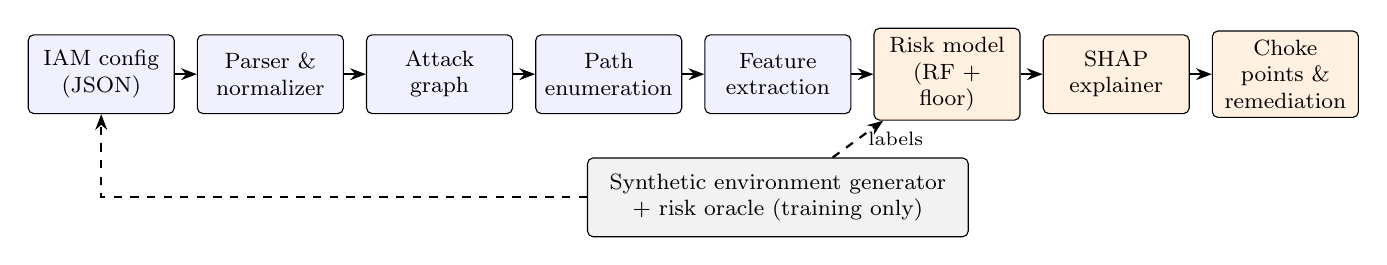
\begin{tikzpicture}[
  node distance=0.28cm,
  box/.style={draw, rounded corners=2pt, align=center, font=\footnotesize,
              minimum height=1.0cm, text width=1.62cm, fill=blue!6},
  ml/.style={box, fill=orange!12},
  arr/.style={-{Stealth[length=2mm]}, thick}]
\node[box] (cfg) {IAM config\\(JSON)};
\node[box, right=of cfg] (parse) {Parser \&\\normalizer};
\node[box, right=of parse] (graph) {Attack\\graph};
\node[box, right=of graph] (paths) {Path\\enumeration};
\node[box, right=of paths] (feat) {Feature\\extraction};
\node[ml, right=of feat] (model) {Risk model\\(RF + floor)};
\node[ml, right=of model] (shap) {SHAP\\explainer};
\node[ml, right=of shap] (choke) {Choke points \&\\remediation};
\foreach \a/\b in {cfg/parse, parse/graph, graph/paths, paths/feat, feat/model, model/shap, shap/choke}
  \draw[arr] (\a) -- (\b);
\node[box, fill=gray!10, below=0.55cm of feat, text width=4.6cm] (gen)
  {Synthetic environment generator + risk oracle (training only)};
\draw[arr, dashed] (gen) -- node[right, font=\scriptsize]{labels} (model);
\draw[arr, dashed] (gen.west) -| (cfg.south);
\end{tikzpicture}
\caption{IAM-XAI pipeline. Blue stages are deterministic graph analysis;
orange stages are learned and explanatory. The generator and oracle are used
only to build training and evaluation data.}
\label{fig:pipeline}
\end{figure*}

Fig.~\ref{fig:pipeline} shows the pipeline. Every stage is a library module
with a command-line entry point, and all randomness is seeded.

\subsection{Parsing and Normalization}
The parser accepts AWS-style IAM JSON (users, groups, roles with trust and
permission policies, resources) in both AWS casing (\code{Effect},
\code{Action}, \code{Statement}) and lower case. It validates structure,
expands single values into lists, and emits a deterministic normalized
representation of entities, permission statements and trust relationships.

\subsection{Attack Graph}
Nodes are users, groups, roles, resources and synthetic principals for
external accounts and the trust wildcard. Directed edges have four types:
\code{CAN\_ASSUME} (a trust policy admits the source and the source holds
\code{sts:AssumeRole}), \code{CAN\_PASS\_ROLE}, \code{CAN\_ACCESS} (read
actions on a resource) and \code{CAN\_MODIFY} (write or policy-changing
actions). Each edge records its actions, resource patterns, conditions and
provenance, so that it can later be mapped to the exact policy statement that
creates it. Explicit \code{Deny} statements remove matching edges. Action-
and resource-aware matching ensures a \code{Deny} on one bucket does not
remove access to another. Conditional denies are conservatively ignored.

\subsection{Attack Path Enumeration}
A depth-first search from every identity enumerates simple (cycle-free) paths
of at most six hops that end at a resource or a passable role. An adjacency
index gives constant-time lookup of outgoing edges. Each path is serialized
with its nodes, edges and hop count.

\subsection{Feature Extraction}
\label{sec:features}
A single shared function turns a path and the analyzer-visible scenario
context into a feature row. Both the dataset generator and the dashboard call
it, and a unit test checks that the two produce identical rows. It
yields 27 fields (Table~\ref{tab:features}); after one-hot encoding the two
categorical fields, the model sees 35 inputs. The context contains only what an
analyst could read from the configuration. This includes resource types, any
\code{DataClassification} tag, which roles hold administrator-equivalent
(\code{*} or \code{iam:*}) permissions, and PassRole targets. It never
contains the true sensitivity of the data.

\begin{table}[t]
\centering
\caption{Per-path feature vector (27 fields)}
\label{tab:features}
\footnotesize
\begin{tabular}{@{}p{1.35cm}p{6.6cm}@{}}
\toprule
Group & Features \\
\midrule
Numeric (12) & path length, role/user/resource count, action count, wildcard-action count, wildcard-resource count, broad-permission edges, conditional edges, condition keys, distinct services, classification tag \\
Binary (13) & assume role, pass role, wildcard action, wildcard resource, policy modification, external trust, cross-account, wildcard principal, sensitive target, admin permission, write access, has conditions, target privileged \\
Categorical (2) & target type, target service \\
\bottomrule
\end{tabular}
\end{table}

\subsection{Risk Models}
We train Logistic Regression (a linear, interpretable baseline), Random Forest
(RF)~\cite{breiman2001rf} and XGBoost~\cite{chen2016xgboost} to predict one of
four classes: LOW, MEDIUM, HIGH or CRITICAL. From the primary model's class
probabilities $P(c \mid \mathbf{x})$ we also derive an \emph{expected risk}
\begin{equation}
  \hat r(\mathbf{x}) = \sum_{c} P(c \mid \mathbf{x})\, w_c, \quad
  w = (0.15,\, 0.40,\, 0.65,\, 0.85),
  \label{eq:exprisk}
\end{equation}
which, unlike the top-class probability, is low for a confident LOW prediction.
It is used to weight paths during choke-point selection.

\textbf{Hybrid model.} Section~\ref{sec:rq2} shows that a learned model cannot
recognize escalation primitives it has never seen. The hybrid model therefore
raises the RF's label to a floor implied by well-known primitives:
administrator-equivalent or policy-modification permissions $\Rightarrow$ at
least HIGH; PassRole of a privileged role $\Rightarrow$ at least HIGH; any
other PassRole $\Rightarrow$ at least MEDIUM. The floor never lowers a label.

\subsection{SHAP Explanations}
For every prediction, TreeExplainer~\cite{lundberg2020tree} computes the SHAP
value $\phi_f$ of each feature $f$ for the predicted class, so that the
features' contributions sum to the difference between that class's
probability and its average over the training data. The top six features by
$|\phi_f|$ form the path's explanation. Because many paths share a feature
vector, SHAP values are computed once per distinct vector. This reduces the
time to explain all 76k paths from roughly three hours to five minutes on a
laptop.

\subsection{Choke-Point Detection and Remediation}
\label{sec:choke}
A choke point is a graph edge, and hence a specific policy statement, whose
removal breaks many high-risk paths. A fixed table maps each model feature to
the edges that carry it. For example, \code{pass\_role} maps to
\code{CAN\_PASS\_ROLE} edges, and \code{external\_trust} maps to
\code{CAN\_ASSUME} edges from external principals. Within a path $p$, edge $e$
receives the score
\begin{equation}
  s_p(e) = 0.1 + 2\!\!\sum_{f \in \mathrm{top}(p),\, f \mapsto e}\!\! |\phi_f|,
\end{equation}
and the highest-scoring edge is the path's own choke point. Across a scenario,
each edge accumulates the expected risk $R(e) = \sum_{p \ni e} \hat r_p$ and the
number of paths $n(e)$ it lies on, and is ranked by
\begin{equation}
  S(e) = R(e)\,\bigl(1 + 0.3\,(n(e) - 1)\bigr) + 0.5\,B(e),
\end{equation}
where $B(e)$ sums $s_p(e)$ over the paths whose own choke point is $e$.
Ranking edges independently can waste cuts on paths that an earlier cut
already broke. For a budget of $k$ cuts we therefore also provide a
\emph{greedy} selector that solves the weighted maximum-coverage problem: it
repeatedly picks the edge on the largest remaining expected risk and then
discards the paths it breaks. The remediation module converts a chosen edge
into a minimal policy diff (removing the action, or the trust statement),
re-runs path discovery on the patched configuration to verify that the paths
are gone, and emits a human-readable playbook.

\subsection{Dashboard}
A local web dashboard runs the entire pipeline on an uploaded or bundled
configuration (Fig.~\ref{fig:dashboard}). It shows the attack graph, per-path
risk, SHAP factors, ranked choke points and one-click remediation with
before/after verification.

\begin{figure*}[t]
\centering
\includegraphics[width=\textwidth]{dashboard.png}
\caption{IAM-XAI dashboard on a generated environment (21 nodes, 25 edges,
13 attack paths). Top: overall posture and counts. Left: attack graph of
users, roles and resources, with choke-point edges in dashed red. Right: SHAP
attribution for the selected CRITICAL path, led by its Secrets Manager target
and data-classification tag.}
\label{fig:dashboard}
\end{figure*}

% ---------------------------------------------------------------------------
\section{Synthetic Dataset and Ground Truth}
\label{sec:dataset}

\subsection{Environment Generator}
Each environment is built from its own seeded random stream, so generation is
reproducible and parallel. It starts from a benign baseline of 3--20 users,
2--15 roles and 5--30 resources of six types: S3 buckets, DynamoDB tables,
Lambda functions, EC2 instances, Secrets Manager secrets and KMS keys. Each
resource has a hidden true data-classification tier: public, internal,
confidential or restricted. Onto this baseline, 0--3 of nine attack patterns
are injected: wildcard action, wildcard resource, PassRole escalation,
AssumeRole chain, external trust, cross-account trust, wildcard trust
(\code{Principal:"*"}), policy modification and administrator wildcard.
Mitigating conditions (MFA, source IP, \code{ExternalId}) and explicit
\code{Deny} guardrails are added at random. Operators' tagging is modeled as
imperfect: 85\% of resources carry a \code{DataClassification} tag, and a few
tags are one tier off.

\subsection{Risk Oracle}
Labels must not be a rule over the model's own features, or learning becomes
circular. The oracle scores each path as
\begin{equation}
  \mathrm{risk} = I \cdot \bigl(0.35 + 0.65\, L\bigr),
  \label{eq:oracle}
\end{equation}
where impact $I$ is the maximum of the reached data's \emph{true} tier impact
(0.10, 0.30, 0.60 and 0.85 from public to restricted, $+0.10$ for write access),
administrator power (0.95), policy-rewrite power (0.90), and PassRole of a
role that is truly privileged (0.90) or not (0.35). Likelihood $L$ is the
exposure of the entry point (wildcard 1.0, external or cross-account 0.9,
internal 0.6), decayed by 0.9 per additional hop and multiplied by a factor
for each \emph{specific} mitigating condition on the path (MFA 0.45, source IP
0.60, \code{ExternalId} 0.65). Cut points 0.20, 0.36 and 0.55 map the score to
LOW, MEDIUM, HIGH and CRITICAL. The oracle also records a human-readable cause
such as \code{restricted\_data + external\_trust}.

The model sees only partial evidence of the oracle's inputs: an imperfect
tag instead of the true tier, whether \emph{some} condition exists instead
of which one, and so on. Identical feature vectors can therefore carry different labels, which
makes the task non-trivial and gives it a measurable ceiling.

\subsection{Dataset}
We generate 3,000 environments. To stop dense environments from
dominating, each is capped at 30 paths with class-balanced sampling. The
result is 76,479 paths (25.5 per environment on average) with 2,068 distinct
feature vectors. The classes are roughly balanced: LOW 20,049, MEDIUM 21,929,
HIGH 19,598 and CRITICAL 14,903. The best accuracy any classifier can reach on
these features, predicting the majority label of each distinct vector, is 0.891.

% ---------------------------------------------------------------------------
\section{Evaluation Protocol}
\label{sec:setup}

\textbf{Splits.} Data are split 70/15/15 into train, validation and test sets
\emph{grouped by environment}, so that no environment contributes paths to
two splits. The random seed is fixed at 42.

\textbf{Tuning.} Models are implemented with scikit-learn~\cite{pedregosa2011sklearn}
and XGBoost. A small grid per model (Logistic Regression: $C$; RF with
300 trees: maximum depth, minimum leaf size, class weighting; XGBoost with
300 rounds: depth, learning rate) is searched on validation macro F1. The
chosen configuration is refit on train+validation and evaluated once on test.

\textbf{Metrics and statistics.} We report accuracy, macro F1, one-vs-rest
ROC-AUC and the \emph{severe-miss rate}: the share of truly HIGH or CRITICAL
paths rated LOW or MEDIUM, the error that matters most to a defender. 95\%
confidence intervals come from 1,000 bootstrap resamples of test
\emph{environments}~\cite{efron1993bootstrap}; model pairs are compared with
McNemar's test~\cite{mcnemar1947,dietterich1998tests}; grouped 5-fold
cross-validation measures stability.

\textbf{Baseline.} A static rule set assigns LOW to read-only access, MEDIUM
to wildcards, HIGH to PassRole, role chains, long paths or sensitive targets,
and CRITICAL to administrator, external or cross-account trust, policy
modification, or a wildcard reaching a sensitive target. It represents
conventional rule-based scoring.

\textbf{Research questions.}
RQ1: How accurately is risk predicted on unseen environments?
RQ2: Are attack patterns never seen in training recognized?
RQ3: Are SHAP explanations correct and faithful?
RQ4: Does cutting IAM-XAI's choke points remove real risk?
RQ5: Do conclusions depend on the oracle's assumptions?
RQ6: Are independently documented attacks detected?

% ---------------------------------------------------------------------------
\section{Results}
\label{sec:results}

\subsection{RQ1: Risk Prediction on Unseen Environments}

\begin{table}[t]
\centering
\caption{Test results on held-out environments (RQ1). Brackets: 95\% bootstrap CI.}
\label{tab:rq1}
\footnotesize
\setlength{\tabcolsep}{3pt}
\begin{tabular}{@{}lcccc@{}}
\toprule
Model & Accuracy & Macro F1 & AUC & Sev.\ miss \\
\midrule
Static rules & 0.421 & 0.390 [.371,.409] & -- & 13.5\% \\
Logistic Reg. & 0.753 & 0.765 [.753,.776] & 0.914 & 12.9\% \\
Random Forest & 0.879 & 0.881 [.870,.891] & 0.974 & \textbf{9.8\%} \\
XGBoost & \textbf{0.882} & \textbf{0.884} [.874,.894] & \textbf{0.979} & 10.4\% \\
Hybrid (RF+floor) & 0.878 & 0.880 [.869,.890] & -- & \textbf{9.8\%} \\
\midrule
\multicolumn{5}{@{}l}{Label-ambiguity ceiling (accuracy): 0.891} \\
\bottomrule
\end{tabular}
\end{table}

Table~\ref{tab:rq1} shows that both tree ensembles come within about 0.01 of
the 0.891 ceiling, so they have learned almost everything the features reveal
about the oracle. Grouped 5-fold cross-validation agrees (macro F1: RF
$0.884\pm0.004$, XGBoost $0.889\pm0.003$, Logistic Regression
$0.754\pm0.003$). XGBoost's advantage over RF is statistically detectable
(McNemar $p=0.005$; 93 vs.\ 58 discordant paths) but smaller than 0.01. We
keep RF as the primary model because it has the lowest severe-miss rate.
Logistic Regression trails by 0.12 macro F1, which indicates that risk depends on
feature interactions, for instance that a sensitive target matters much more
when the entry point is external. The static rules reach only 0.390 macro F1.
They are too coarse, because a single wildcard or PassRole flag does not
determine risk once exposure and mitigating conditions are accounted for. On the
11,526 test paths the hybrid floor turns 9 correct RF predictions into
over-estimates and corrects none (McNemar $p=0.004$), an accuracy cost of 0.001. Fig.~\ref{fig:confusion} shows that most RF errors fall
between adjacent classes.

\begin{figure}[t]
\centering
\includegraphics[width=0.85\columnwidth]{fig2_confusion_matrix.png}
\caption{Random Forest confusion matrix on the test environments. Most errors are between adjacent risk levels.}
\label{fig:confusion}
\end{figure}

\subsection{RQ2: Attack Patterns Never Seen in Training}
\label{sec:rq2}
For each of the nine attack patterns we train the RF only on environments
\emph{without} that pattern and test it on held-out paths that exercise it.
Fig.~\ref{fig:lopo} shows the severe-miss rates. \emph{Structural} patterns
transfer well, because they combine features the model has seen in other
contexts: assume-role chains, wildcard actions and resources, and
external or cross-account trust (severe-miss 1.3--14.3\%). Escalation
\emph{primitives} do not. With no PassRole example in training, the RF rates
96.8\% of severe PassRole paths LOW or MEDIUM, and it misses 57.9\% of
administrator-wildcard paths. A learned model cannot infer that a permission
it has never seen grants administrator power. The hybrid floor encodes this
domain knowledge and brings the severe-miss rate for PassRole, administrator
wildcard and policy modification to 0\%, while leaving in-distribution
accuracy unchanged (RQ1). Wildcard trust (\code{Principal:"*"}) remains the
hardest structural pattern at 22.0\%; unlike the primitives above, it is
not covered by the floor and is a candidate for a further domain rule.

\begin{figure}[t]
\centering
\includegraphics[width=\columnwidth]{fig3_unseen_pattern_generalization.png}
\caption{Leave-one-pattern-out severe-miss rate (RQ2). The escalation floor
eliminates misses on the three privilege-escalation primitives.}
\label{fig:lopo}
\end{figure}

\subsection{RQ3: Correctness and Faithfulness of Explanations}
We sample 3,000 test paths and ask two questions. \emph{Correctness}: do the
top SHAP features name the oracle's true drivers of risk? Each cause term,
such as \code{restricted\_data} or \code{external\_trust}, is mapped to the
feature group that can reveal it. \emph{Faithfulness}: do the features SHAP
ranks highest actually drive the model? We reset the top-$k$ features to their
training medians and measure the drop in the predicted class's
probability~\cite{samek2017evaluating}. The baselines are a single global ranking
(mean $|\phi|$ over all evaluated paths) and a random ranking.

\begin{table}[t]
\centering
\caption{Explanation correctness and faithfulness (RQ3, 3,000 test paths)}
\label{tab:rq3}
\footnotesize
\setlength{\tabcolsep}{2.6pt}
\begin{tabular}{@{}lccccc@{}}
\toprule
& \multicolumn{3}{c}{True cause recovered} & \multicolumn{2}{c}{Prob.\ drop} \\
\cmidrule(lr){2-4}\cmidrule(l){5-6}
Ranking & Top-1 & Top-3 & Top-3 multi & $k{=}1$ & $k{=}3$ \\
\midrule
SHAP (per path) & \textbf{95.3\%} & \textbf{90.5\%} & \textbf{77.0\%} & \textbf{0.387} & \textbf{0.537} \\
Global importance & 95.0\% & 84.5\% & 70.6\% & 0.299 & 0.427 \\
Random & 29.9\% & 52.8\% & 38.4\% & 0.021 & 0.066 \\
\bottomrule
\end{tabular}
\end{table}

Table~\ref{tab:rq3} shows that the top SHAP feature names a true cause for
95.3\% of paths. The global ranking does almost as well at top-1, because the
target's data classification is the dominant cause for most paths. The
per-path explanations pull ahead where it matters. On paths with several
causes they recover 77.0\% of the true causes in their top three, against
70.6\% for the global ranking. Removing SHAP's top three features lowers the
model's confidence by 0.537, against 0.427 for the global ranking and 0.066
for a random one. The explanations therefore reflect what the model actually
uses. Fig.~\ref{fig:waterfall} shows a typical CRITICAL path. The
restricted-data tag and sensitive target dominate, and external trust, a
wildcard action and cross-account access add smaller contributions.

\begin{figure}[t]
\centering
\includegraphics[width=\columnwidth]{shap_waterfall_example.png}
\caption{SHAP waterfall for a path predicted CRITICAL: a principal from an external account reaches a restricted resource with a wildcard action.}
\label{fig:waterfall}
\end{figure}

\subsection{RQ4: Choke-Point Remediation}
We generate 200 fresh environments with a seed never used in training (6,979
paths). We cut $k$ edges chosen by each strategy and measure the share of
\emph{ground-truth oracle} risk removed. The strategies are a random edge,
the most-shared edge (pure graph topology), IAM-XAI's ranking
$S(e)$, the same ranking without the SHAP term (ablation), the greedy
selector, and an upper bound that runs greedy with the hidden oracle scores.

\begin{table}[t]
\centering
\caption{Ground-truth risk removed by cutting $k$ edges (RQ4, 200 unseen environments)}
\label{tab:rq4}
\footnotesize
\setlength{\tabcolsep}{3pt}
\begin{tabular}{@{}lccc@{}}
\toprule
Strategy & Risk, $k{=}1$ & Risk, $k{=}3$ & Severe paths, $k{=}3$ \\
\midrule
Random edge & 7.2\% & 20.0\% & 20.8\% \\
Most-shared edge & 24.6\% & 43.9\% & 43.9\% \\
IAM-XAI ranked & 25.8\% & 46.6\% & 50.1\% \\
\quad ranked, no SHAP & 26.0\% & 46.7\% & 49.5\% \\
IAM-XAI greedy & \textbf{26.4\%} & \textbf{52.3\%} & \textbf{59.7\%} \\
\midrule
Oracle upper bound & 26.7\% & 52.7\% & 61.3\% \\
\bottomrule
\end{tabular}
\end{table}

With three cuts, greedy selection removes 52.3\% of real risk and 59.7\% of
severe paths (Table~\ref{tab:rq4}). This is 99\% of the oracle optimum, and
7.3--9.7 percentage points more than the graph-only baseline (95\% paired
bootstrap CI). The ablation clarifies where the gain comes from. Removing the
SHAP term from the ranking changes almost nothing, so the improvement over
pure topology comes from \emph{ML risk weighting}, and the gain of greedy over
ranked selection comes from avoiding redundant cuts. SHAP's role in remediation
is to explain \emph{why} an edge matters to the engineer who must approve its
removal, not to select it. We report this as a finding, not a weakness: it
separates the value of prediction from the value of explanation.

\subsection{RQ5: Sensitivity to Oracle Assumptions}

\begin{table}[t]
\centering
\caption{Macro F1 under perturbed oracles (RQ5, 1,500 environments each)}
\label{tab:rq5}
\footnotesize
\setlength{\tabcolsep}{3.5pt}
\begin{tabular}{@{}lccccc@{}}
\toprule
Variant & Ceiling & Rules & LR & RF & Hybrid \\
\midrule
Default & 0.890 & 0.378 & 0.755 & 0.875 & 0.875 \\
Label noise 5\% & 0.848 & 0.370 & 0.730 & 0.834 & 0.834 \\
Label noise 10\% & 0.807 & 0.366 & 0.705 & 0.788 & 0.788 \\
Weights perturbed (a) & 0.897 & 0.378 & 0.775 & 0.886 & 0.886 \\
Weights perturbed (b) & 0.912 & 0.448 & 0.796 & 0.918 & 0.918 \\
Weights perturbed (c) & 0.888 & 0.389 & 0.747 & 0.871 & 0.871 \\
Cut points $-10\%$ & 0.878 & 0.388 & 0.770 & 0.863 & 0.863 \\
Cut points $+10\%$ & 0.920 & 0.453 & 0.769 & 0.905 & 0.905 \\
\bottomrule
\end{tabular}
\end{table}

Because our labels come from an oracle we designed, we check whether the
conclusions depend on its specific numbers. Each variant regenerates 1,500
environments with injected label noise, randomly perturbed oracle weights
($\pm 20\%$) or cut points shifted by $\pm 10\%$, and retrains all models
(Table~\ref{tab:rq5}). In every variant the ordering RF $>$ Logistic
Regression $\gg$ static rules holds. RF macro F1 stays within 0.02 of the
variant's accuracy ceiling, and the hybrid's severe-miss rate stays between
7.2\% and 12.5\%. Label noise lowers the ceiling and every model with it, as
expected.

\subsection{RQ6: Independently Documented Attacks}
To check that IAM-XAI is not merely learning its own generator, we encode
32 hand-written configurations and run them through the unchanged pipeline.
Twenty-one are the IAM privilege-escalation methods catalogued by Rhino
Security Labs~\cite{gietzen2018rhino}. Five are modeled on CloudGoat
scenarios~\cite{cloudgoat} and well-known trust misconfigurations, for example
cross-account trust without an \code{ExternalId}.
Six are benign controls. An attack counts as detected if any of its paths is
rated HIGH or CRITICAL.

\begin{table}[t]
\centering
\caption{External benchmark (RQ6)}
\label{tab:rq6}
\footnotesize
\begin{tabular}{@{}lcc@{}}
\toprule
Method & Attacks detected & False alarms (benign) \\
\midrule
Random Forest & 18/26 (69\%) & 0/6 \\
Hybrid & 18/26 (69\%) & 0/6 \\
Static rules & 18/26 (69\%) & 0/6 \\
\bottomrule
\end{tabular}
\end{table}

Attack paths were found for all 26 attack scenarios, and 18 were rated HIGH or
CRITICAL with no false alarm on the benign controls (Table~\ref{tab:rq6}).
The detection counts are equal across methods, but the learned models grade
more precisely. They rate every PassRole-based attack (R03, R15, R16, R18, R20,
R21 and CloudGoat-style C02, C03) CRITICAL where the rules say HIGH. They rate
a public-trust role reading restricted data (C05) CRITICAL, and a write
blocked by an explicit \code{Deny} (N06) LOW where the rules say MEDIUM. The
eight misses share one cause: the attack graph does not yet model their
escalation mechanism. These mechanisms are taking over another user's
credentials (\code{iam:CreateAccessKey}, \code{CreateLoginProfile},
\code{UpdateLoginProfile}), joining a group (\code{iam:AddUserToGroup}),
rewriting the policy of a role the attacker can already assume
(\code{AttachRolePolicy}, \code{PutRolePolicy}), and injecting code into a
privileged service (\code{lambda:UpdateFunctionCode},
\code{glue:UpdateDevEndpoint}). We deliberately did not patch the graph after
seeing these results, to avoid tuning on the benchmark. They define the next
set of edge types to add.

% ---------------------------------------------------------------------------
\section{Discussion and Threats to Validity}
\label{sec:discussion}

\textbf{What the results mean.} On the features an analyzer can extract, a tree
ensemble approximates a principled impact$\times$likelihood risk model almost
perfectly, and it far outperforms fixed rules. Explanations name true causes
and are faithful to the model. Risk-weighted choke-point selection
approaches the optimum. The most practically important result is RQ2. A
purely data-driven risk model is blind to escalation primitives outside its
training distribution, and a few lines of domain knowledge fix this at no
measurable cost. We recommend that learned IAM risk scoring always be paired
with such a floor.

\textbf{Synthetic ground truth.} The models learn our oracle, not expert
judgment about real incidents. We mitigate this in four ways: the oracle
follows the standard risk $=$ impact $\times$ likelihood
decomposition of NIST SP 800-30~\cite{nist2012sp80030} rather than a severity score
such as CVSS~\cite{first2019cvss31}, it uses information the model sees only
partially, conclusions hold under perturbed weights, noise and cut points
(RQ5), and detection is checked against independently published attacks
(RQ6). A study with expert-labeled real configurations remains necessary.

\textbf{Low-cardinality features.} 98.2\% of test feature vectors also occur
in training. Grouped splits prevent environment-level leakage, and the ceiling
bounds achievable accuracy, but RQ1 measures generalization to new
environments more than to new feature combinations. RQ2 and RQ6 test the latter.

\textbf{Graph coverage and scale.} Credential takeover, group-membership
changes and code injection are not modeled (RQ6). Path enumeration is
exponential in dense graphs. Our synthetic environments are laptop-scale, and
large enterprise accounts will need pruning or streaming enumeration.

\textbf{Remediation feasibility.} RQ4 assumes any edge can be cut without
business impact. In practice some permissions are required, and a
\code{CAN\_ASSUME} patch currently revokes the whole trust statement instead of
a single principal.

\textbf{Explanation mapping.} Mapping causes to features for RQ3 was
defined by the authors. The random baseline shows that the mapping is not
trivially satisfied, but other mappings could shift the absolute numbers.

% ---------------------------------------------------------------------------
\section{Conclusion and Future Work}
\label{sec:conclusion}

IAM-XAI turns an IAM configuration into ranked, explained and remediable
privilege-escalation paths. On 3,000 synthetic environments with
non-circular ground truth, a Random Forest predicts path risk at 0.881 macro
F1, near the 0.891 ceiling and far above static rules (0.390). SHAP
explanations recover true causes for 95\% of paths and are faithful to the
model. Three greedily chosen cuts remove 52.3\% of real risk, 99\% of the
optimum. A domain-knowledge floor removes the blind spot of learned models on
unseen escalation primitives. On 26 published attacks the pipeline detects 18
with no false alarms, and every miss traces to a known, documented gap in
graph coverage.

Future work will (i) add edge types for credential takeover, group membership,
role-policy rewriting and code injection, and evaluate them on a
\emph{fresh} set of techniques such as the 31 IAM Vulnerable
scenarios~\cite{iamvulnerable}; (ii) validate risk labels against expert
judgment on real, anonymized configurations; (iii) model the business cost of
removing a permission in choke-point selection; and (iv) scale path
enumeration to enterprise-size accounts. All code, data, trained models and
results are reproducible from a single set of commands and are publicly
available at \url{https://github.com/alan61503/IAM-XAI}.

\section*{Acknowledgment}
The authors thank Dr.\ Julian Benedit P for guidance throughout this work, and the Department
of Computer Science and Engineering, CHRIST (Deemed to be University), for its
support.

\bibliographystyle{IEEEtran}
\bibliography{refs}

\end{document}
